\section{Ziel}
\label{sec:Ziel}
In diesem Versuch soll der Temperaturverlauf der Molwärme von 
Kupfer untersucht werden. Die gemessenen Werte werden mit dem 
Dulong-Petit-Modell, dem Einstein-Modell und dem Debye-Modell 
verglichen.

\section{Theorie}
\label{sec:Theorie}
Bei der Wärmekapazität eines Stoffes handelt es sich um die Wärmemenge $\increment Q$, die 
man ihm zufügen muss, um eine gewisse Temperaturänderung $\increment T$ zu erzielen:
\begin{equation*}
    C = \frac{\increment Q}{\increment T}.
\end{equation*}
Diese Größe kann auf die Masse, das Volumen oder der Stoffmenge einer Probe bezogen werden. 
In diesem Versuch wird die molare Wärmekapazität, auch Molwärme genannt, untersucht, die sich über 
\begin{equation*}
    c^{\si{m}} = \frac{C}{\si{mol}}
\end{equation*}
aus der Wärmekapazität berechnet. 

Die Molwärme hängt davon ab, ob man sie bei konstantem Druck $P$ oder konstantem Volumen $V$ der Probe betrachtet. Da bei einem nicht konstantem Volumen 
Energie für die Ausdehnung des Stoffes benötigt wird, ist die Molwärme bei konstantem Druck $C_{\si{P}}$ größer als die Molwärme bei konstantem Volumen $C_{\si{V}}$. 
Da der Druck leichter konstant zu halten ist als das Volumen, wird meistens die Molwärme bei konstantem Druck gemessen. 
Die beiden Werte lassen sich aber über die Beziehung 
\begin{equation}
    \label{eqn:cv}
    C_{\si{V}}=C_{\si{P}}-9\alpha ^2 \kappa  V_0 T
\end{equation}
ineinander umrechnen. Hier ist $\alpha$ der Ausdehnungskoeffizient, der in einer Tabelle abgelesen werden kann, $\kappa$ das Kompressionsmodul
und $V_0$ das Molvolumen. Der Unterschied zwischen den Molwärmen ist bei Festkörpern nur gering, da sie sich nur wenig ausdehnen.
\\

Da in diesem Versuch die Wärmeenergie mit einem über ein Zeitintervall $t$ angeschlossenen Heizstrom $I$ zugeführt wird, 
berechnet sich die Molwärme über
\begin{equation}
    \label{eqn:cp}
    C_{\si{p}} = \frac{M}{m} \frac{U\cdot I \cdot t}{\increment T},
\end{equation}
wobei $U$ die Heizspannung, $M$ die molare Masse und $m$ die Masse der Probe ist.
\\

Nach klassischer Betrachtung ist die Molwärme konstant $3R$, wobei $R$ die allgemeine Gaskonstante ist. Das nennt sich Dulong-Petit-Gesetz. 
Demnach wäre die Molwärme unabhängig von der Temperatur für alle Stoffe gleich. 
Im Experiment zeigt sich jedoch, dass die Molwärme für tiefe Temperaturen stark davon abweicht, aber sich für 
hohe Temperaturen an den Dulong-Petit-Wert annähert. Die Molwärme zeigt für tiefe Temperaturen eine $T^3$-Abhängigkeit. 


Das kann mit der Quantenmechanik erklärt werden, indem die Gitterschwingungen des Kristallgitters 
berücksichtigt werden. Ein quantenmechanischer harmonischer Oszillator kann nur bestimmte Energiebeträge aufnehmen, 
denn es sind nur die Energiewerte $ E_{\si{n}} = (n+\frac{1}{2}) \hbar \omega $ möglich. Ist die Wärmeenergie $k_{\si{B}}T$ mit der Boltzmann-Konstant $k_{\si{B}}$
nun viel kleiner als $\hbar\omega$, kann dieser Energiebetrag nicht mehr aufgenommen werden. 
Da in einem Kristall verschiedene Eigenfrequenzen $\omega$ vorkommen, werden mit sinkender Temperatur nach und nach immer weniger 
Oszillatoren die Wärmeenergie aufnehmen können. Dadurch wird die Energie, die für eine Temperaturerhöhung nötig ist, größer. 
\\

Zur Beschreibung des Temperaturverlaufs bei tieferen Temperaturen gibt es zwei Modelle, das Einstein- und das Debye-Modell. 
Die Phonon-Dispersion eines Festkörpers mit einatomiger Basis sieht schematisch wie in Abbildung \ref{fig:2} aus. 
\FloatBarrier
\begin{figure}
  \centering
  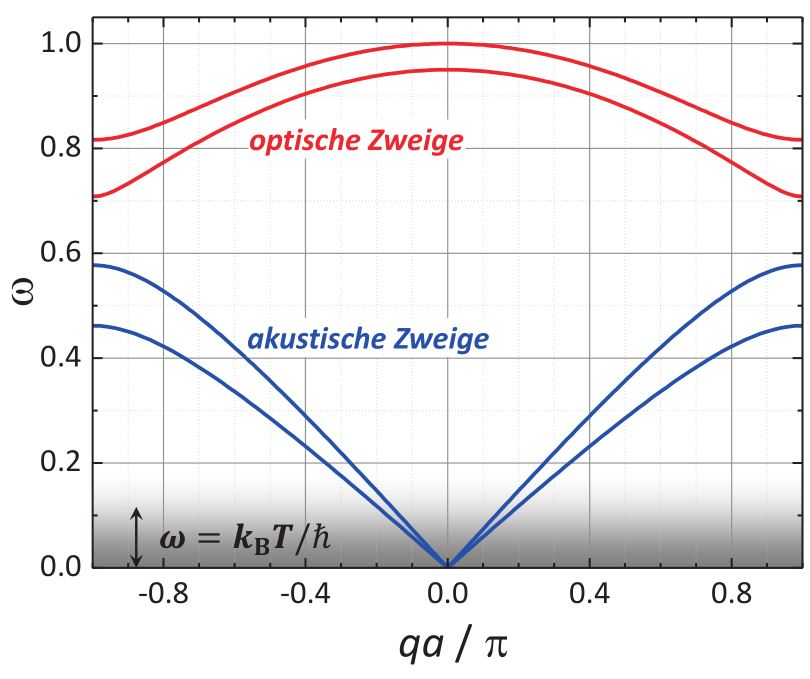
\includegraphics[width=0.55\textwidth]{2.JPG}
  \caption{Phonon-Dispersion eines Festkörpers [2].}
  \label{fig:2}
\end{figure}
\FloatBarrier
Im Einstein-Modell werden die optischen Phononen auf eine Gerade genähert,
im Debye-Modell die akustischen Phononen auf zwei Geraden. Da bei hohen Temperaturen die optischen Phononen dominieren,
eignet sich hierfür die Beschreibung durch das Einstein Modells. Umgekehrt gelingt die Beschreibung der Molwärme für tiefe Temperaturen mit dem Debye-Modell besser.
\\

Im Einstein-Modell wird angenommen, dass alle $3N$-Eigenschwingungen des Kristallgitters die gleiche
Eigenfrequenz $\omega_{\si{E}}$ haben. Dadurch ergibt die Funktion der Wärmekapazität eine e-Funktion. 
Für hohe Temperaturen nähert sich das Modell dem Dulong-Petit-Gesetz an. 
\\ 

Beim Debye-Modell wird hingegen angenommen, dass die Frequenzverteilung einer Parabel entspricht. Die Debye-Näherung 
im Vergleich zur realen Frequenzverteilung ist in Abbildung \ref{fig:3} dargestellt.
\FloatBarrier
\begin{figure}
  \centering
  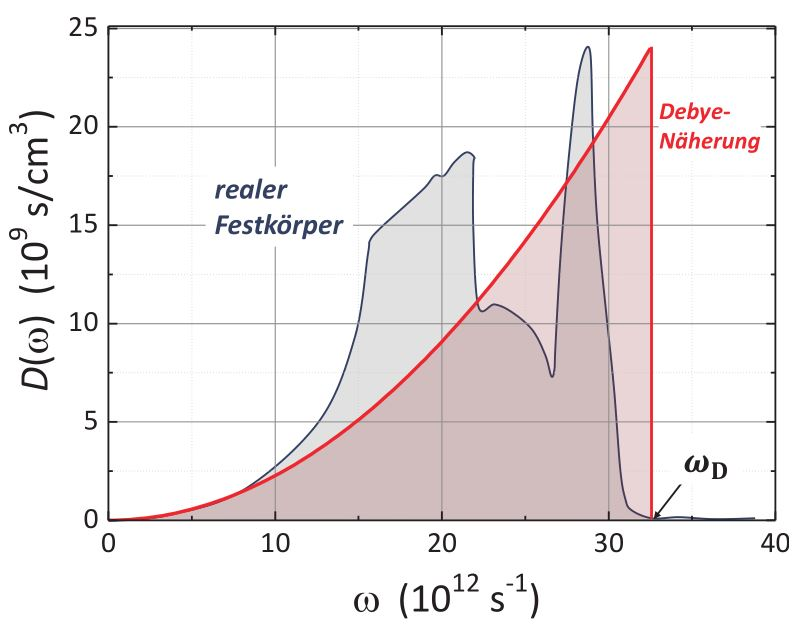
\includegraphics[width=0.55\textwidth]{3.JPG}
  \caption{Reale Phononenzustandsdichte im Vergleich zur Debye-Näherung [2].}
  \label{fig:3}
\end{figure}
\FloatBarrier
Hierbei ist die Debye-Frequenz $\omega_{\si{D}}$ so gewählt, dass die 
Flächen unter den Kurven gleich groß sind. Sie kann über die Formel 
\begin{equation}
    \label{eqn:wd}
    \omega_{\si{D}} = \sqrt[3]{\frac{18 \si{\pi}^2 N_{\si{A}}}{V_0}\left(\frac{1}{v_{\si{long.}}^3}+\frac{2}{v_{\si{trans.}}^3}\right)^{-1}}
\end{equation}
bestimmt werden, wobei $N_{\si{A}}$ die Avogadrokonstante ist. 
Die Debye-Temperatur $\theta_{\si{D}}$ berechnet sich dann über
\begin{equation}
    \label{eqn:dT}
    \theta_{\si{D}} = \frac{\hbar \omega_{\si{D}}}{k_{\si{B}}}
\end{equation}

Es ergibt sich ein Temperaturverlauf mit $T^3$-Abhängigkeit für niedrige Temperaturen und 
das Dulong-Petit-Gesetz für hohe Temperaturen.


